% Copyright 2018-2021 Melvin Eloy Irizarry-Gelpí
\setcounter{chapter}{1}
\chapter{Factors Affecting Electrical Resistance}
%
In this experiment you will learn about electrical resistance and resistivity.
%
\section{Preliminary}
%
At the microscopic level, the sources of electric charge are inside atoms. You have the \textbf{electron cloud}, with \textbf{negative} charges, and the \textbf{nucleus}, with \textbf{positive} charges (and also neutral charges that help keep the nucleus together). The atoms inside a typical piece of solid matter are arranged in a way such that the nuclei are held in place and do not move much but the electrons can jump to other atoms. In this sense, electric charge can flow through a material.

How easy it is for electrons to jump between atoms depends on how the atoms in a solid are arranged, and on how tightly the atom is holding on to the electron cloud. Depending on your goal, you might want to use a material that allows charges to move more easily (e.g. if you want to add wiring to your home). Electrical \textbf{resistance} and \textbf{resistivity} are two quantities that allow you to quantify and compare the ease of electric charge flow through a material. Before introducing the units used to measure these two quantities, it is useful to briefly mention other important electrical quantities.

Recall that the SI unit for \textbf{electric charge} is the \textbf{coulomb} (C). The coulomb is a derived unit that is defined in terms of other SI units, like the ampere and the second.
%
\subsection{Electric Potential and Voltage}
%
The Coulomb force can turn electric potential energy into work. The SI unit for \textbf{energy} is the \textbf{joule} (J). The amount of electric potential energy per unit of electric charge is known as the \textbf{electric potential}. Since energy is in J and electric charge is in C, the unit for electric potential is J/C. This combination of units is known as a \textbf{volt} (symbol is V):
\begin{equation}
	1 \ \text{volt} = 1 \ \text{V} = 1 \ \text{J/C} = 1 \ \text{joule per coulomb}
\end{equation}
The volt is the \textbf{SI unit} for electric \textbf{potential}. Electric potential, like energy, does not have a direction associated to it. Every point in space has a value of electric potential. If point 1 in space has an electric potential of $V_{1}$ and point 2 in space has an electric potential of $V_{2}$, then we say that there is a voltage $\Delta V$ given by
\begin{equation}
	\Delta V = V_{2} - V_{1}
\end{equation}
That is, a \textbf{voltage} is a difference of electric potential between two points in space. Technically speaking, absolute electric potential is not directly measurable, but voltage is.

The mathematical symbol for electric potential is $V$.
%
\subsection{Electric Current}
%
Another important quantity is \textbf{electric current}. Electric current quantifies the rate of flow of electric charge with respect to time (through a point in space). Since electric charge is in coulombs and time is in seconds, the \textbf{SI unit} for electric \textbf{current} is C/s. This combination of units is known as an \textbf{ampere} (symbol is A):
\begin{equation}
	1 \ \text{A} = 1 \ \text{C/s}
\end{equation}
Although flow of charge in space suggests a direction is involved, the electric current is \textbf{not a vector} quantity.

The mathematical symbol for electric current is $I$.
%
\subsection{Electrical Resistance}
%
After introducing electric potential and electric current, and the units used to measure these quantities, you are ready to formally discuss \textbf{electric resistance}. The point of electric resistance is to quantify how easy it is for a current to flow through a particular material. The \textbf{SI unit} for electrical \textbf{resistance} is the \textbf{ohm} (symbol is $\Omega$, the uppercase Greek letter omega). Electric resistance is not a fundamental quantity. The ohm unit can be stated in terms of volts and amps:
\begin{equation}
	1 \ \text{ohm} = 1 \ \text{V/A}
\end{equation}
This result suggests that electrical resistance can be found by taking an electric potential value, and dividing it by an electric current value.

When a piece of material has a large value of electrical resistance, it means that it is harder to get an electric current to flow through that piece of material. Small values of electrical resistance mean that it is easier for electric current to flow.

The mathematical symbol for electrical resistance is $R$.
%
\subsection{Ohm's Law}
%
Many materials, but not all of them, satisfy \textbf{Ohm's law}: the amount of electric potential difference $V$ across a piece of material is directly proportional to the amount of electric current $I$ flowing through the material:
\begin{equation}
	V = IR
\end{equation}
As you can see, the factor of proportionality in this relation is a quantity with units of electrical resistance, and indeed corresponds to the electric resistance of the material. When such a relation holds, the material is said to be \textbf{ohmic}. For ohmic materials, the electrical resistance $R$ can be found from the slope of the voltage versus current chart. In general, if you know the current and voltage values, you can calculate resistance via
\begin{equation}
	R = \frac{V}{I}
	\label{eq.02.ohms.law}
\end{equation}
Not all materials are ohmic.
%
\subsection{Geometry of a Cylinder}
%
Each distinct material has its own value of electrical resistance. As you will find during this experiment, electrical resistance not only depends on the kind of material being use, but also on the \textbf{geometrical} aspects of the particular piece of material under study.

To a good approximation, almost all electrical wires have a cylindrical shape. A \textbf{cylinder} is a shape with a \textbf{length} $l$ and a circular base with \textbf{area} $A$. The area of a circle is
\begin{equation}
	A = \frac{1}{4} \pi d^{2}
	\label{eq.02.area}
\end{equation}
Here $d$ is the \textbf{diameter} of the circular base. Recall that the diameter of a circle is twice its radius, and that the radius of a circle is the distance from the center of the circle to any point on the circle. It turns out that the electrical resistance of a cylindrical wire depends on the length $l$ and the area $A$ of the cylinder.
%
\subsection{Electrical Resistivity}
%
For convenience, it is useful to introduce a quantity called \textbf{electrical resistivity} that is similar to electrical resistance, but does not depend on the geometrical aspects of the particular piece of material. In this way, electrical resistivity is \textbf{more intrinsic} than electrical resistance. The \textbf{SI unit} for electrical resistivity is the ohm{ }\textperiodcentered{ }meter (i.e. ohm multiply by meter).

The mathematical symbol for electrical resistivity is $\rho$ (the lowercase Greek letter rho).
%
\section{Experiment}
%
The main goal of this experiment is to study and understand how the electrical resistance $R$ of a cylindrical wire depends on the length $l$ of the wire, and the area $A$ of the cross-section of the wire. In principle, you would measure $R$, $l$, and $A$, and then make a chart. In practice you cannot measure $R$ directly. Instead you measure electric potential and electric current directly, and then use Equation (\ref{eq.02.ohms.law}) to calculate $R$.

You have eight different rods. Four of them are made of brass (but these four brass rods have different diameter), the other four are made of other materials (but these four rods have the same diameter).
%
\subsection{Part 1: Effect of Length}
%
In the first part you keep the material and the cross-sectional area fixed, and consider different lengths:
\begin{itemize}
	\item Run 1: Brass, $d = 3.18$ mm
\end{itemize}
You should consider about six different length values.
%
\subsection{Part 2: Effect of Material}
%
In the second part you change the material, but keep the cross-sectional area fixed, and consider different lengths for each material:
\begin{itemize}
	\item Run 2: Copper, $d = 3.18$ mm
	\item Run 3: Music Wire, $d = 3.18$ mm
	\item Run 4: Aluminum, $d = 3.18$ mm
	\item Run 5: Stainless Steel, $d = 3.18$ mm
\end{itemize}
For each material you should consider six different length values.
%
\subsection{Part 3: Effect of Cross-Sectional Area}
%
In the third part you keep the material fixed, and consider different cross-sectional areas:
\begin{itemize}
	\item Run 6: Brass, $d = 2.38$ mm
	\item Run 6: Brass, $d = 3.97$ mm
	\item Run 8: Brass, $d = 4.76$ mm
\end{itemize}
For each rod you should consider six different length values.
%
\section{Analysis}
%
Many \textbf{non-SI units} are used in this experiment, mostly for convenience reasons:
\begin{itemize}
	\item Length along the rod is in centimeters (cm).
	\item Diameter of the rod is in millimeters (mm).
	\item Electric potential along rod segment is in millivolts (mV).
\end{itemize}
Recall that
\begin{align}
	1 \ \text{cm} = 0.01 \ \text{m} && 1 \ \text{mm} = 0.001 \ \text{m} && 1 \ \text{mV} = 0.001 \ \text{V}
\end{align}
It is very important that SI units are used before any calculations, so that the resistance comes out in ohm units and the resistivity comes out in ohm{ }\textperiodcentered{ }meter units.
%
\subsection{Part 1 and Part 2: Length}
%
Here is what to do for runs 1, 2, 3, 4, and 5.
%
\subsubsection{Convert the units of potential to SI units}
%
The LabQuest device will measure the electric potential in units of millivolts (mV). In a separate column, convert these values to units of volts (V) by multiplying each millivolt value by a factor of 0.001.
%
\subsubsection{Calculate the resistance in ohms}
%
With the current in amps, and the potential in volts, you can calculate the resistance in ohms by using (\ref{eq.02.ohms.law}).
%
\subsubsection{Convert the units of length to SI units}
%
You used the centimeter (cm) marks to measure the length along the rod where the electric potential measurement was taken. In a separate column, convert these values to units of meters (m) by multiplying each centimeter value by a factor of 0.01.
%
\subsubsection{Make a chart of $R$ versus $l$}
%
It is time to visualize the data. Make a \textbf{scatter chart} with resistance in the vertical axis, and length in the horizontal axis. Label both axes and add a title to each chart that includes the run number, the material being used, and the value of the diameter.
%
\subsubsection{Calculate the slope of the best-fit line}
%
If the shape of the data is linear, include a \textbf{best-fit line}. In a separate cell, use the \texttt{SLOPE} function to calculate the value of the slope. If the linear fit is appropriate, this suggest that the amount of resistance $R$ is directly proportional to the amount of length $l$:
\begin{equation}
	R = a_{1} l + b_{1}
\end{equation}
Here, $a_{1}$ is the slope and $b_{1}$ is the intercept. The slope $a_{1}$ should have ohm/m units, and the intercept $b_{1}$ should have ohm units.

Note that the cross-sectional area $A$ was kept constant.
%
\subsection{Part 3: Area}
%
For runs 6, 7, and 8 you should do the same steps as those for the previous runs. Along with run 1, for each length value you should have four values for resistance and area. Here is what to do after you have the resistance versus length values.
%
\subsubsection{Convert the units of diameter to SI units}
%
The diameter of each rod is given in units of millimeters (mm). In a separate column, convert these values to units of meter (m) by multiplying each millimeter value by a factor of 0.001.
%
\subsubsection{Calculate the area in m\textsuperscript{2}}
%
With the diameter in meter units, you can calculate the area using (\ref{eq.02.area}). For $\pi$ you can use \texttt{PI()} instead of writing the value by hand.
%
\subsubsection{Calculate the inverse area in m\textsuperscript{\textminus 2}}
%
It is going to be important to calculate the inverse area. In a separate column, calculate the reciprocal inverse of each area value.
%
\subsubsection{Make a chart of resistance versus inverse area}
%
Choose a length value, then gather the corresponding resistance value from runs 1, 6, 7, and 8. You should have resistance for four different areas (or inverse areas).

If you make a chart with $R$ in the vertical axis, and $A$ in the horizontal axis, you will find that although there is a pattern, it is not a linear pattern (see Figure \ref{figure.02.10cm.non.linear}). Instead, the chart with $R$ in the vertical axis, and $1/A$ in the horizontal axis does show a linear pattern.
%
\subsubsection{Calculate the slope of the best-fit line}
%
A linear shape suggests that $R$ is directly proportional to $1/A$:
\begin{equation}
	R = \frac{a_{2}}{A} + b_{2}
\end{equation}
Here $a_{2}$ is the slope and $b_{2}$ is the intercept. The slope $a_{2}$ should have ohm{ }\textperiodcentered{ }m\textsuperscript{2} units, and the intercept $b_{2}$ should have ohm units.

Note that the length $l$ was kept constant.
%
\subsection{Part 4: Resistivity}
%
Keeping the area fixed and letting the length vary yielded the following linear relation:
\begin{equation}
	R = a_{1} l + b_{1}
\end{equation}
Keeping the length fixed and letting the area vary yielded the following linear relation:
\begin{equation}
	R = \frac{a_{2}}{A} + b_{2}
\end{equation}
Ignoring the intercepts, the two previous equations suggest a relation between resistance, length, and cross-sectional area of the form:
\begin{equation}
	R = a_{3} \frac{l}{A}
\end{equation}
Here $a_{3}$ has ohm{ }\textperiodcentered{ }m units, the same units as resistivity. This suggests that $a_{3}$ corresponds to the resistivity.

You can now go back to your results and compute the resistivity from the $a_{1}$ value by multiplying it by the corresponding area:
\begin{equation}
	\rho = a_{1} A
\end{equation}
Similarly, you can compute the resistivity from the $a_{2}$ value by dividing it by the corresponding length:
\begin{equation}
	\rho = \frac{a_{2}}{l}
\end{equation}
In principle, these two methods of obtaining the resistivity should yield very similar values.
%
\subsection{Comparisons with Established Results}
%
Your experimental results for the electrical resistivity can be compared to established values. See Table \ref{table.02.established}. The values for brass, copper, and aluminum were taken from this \href{http://www.radio-electronics.com/info/formulae/resistance/resistivity-table.php}{website}. The value for stainless steel and music wire was taken from \href{https://en.wikipedia.org/wiki/Electrical_resistivity_and_conductivity}{Wikipedia}. Since some kinds of music wire is made with carbon steel, you can compare the resistivity of music wire to the resistivity of carbon steel.
%
\section{My Data}
%
Keeping the area fixed, you can find the electrical resistivity for each of the eight runs. Table \ref{table.02.experimental.area} contains my results. Each resistivity is found by multiplying the value of the slope from the best-fit line by the corresponding area. For example, Figure \ref{figure.02.run.1} has the data for run 1. The slope is 4.97{ }\texttimes{ }10\textsuperscript{\textminus 3} ohm/m. The diameter is 3.18 mm, giving an area of 7.96{ }\texttimes{ }10\textsuperscript{\textminus 6} m\textsuperscript{2}. The resistivity is
\begin{equation}
	\rho = \left(4.97 \times 10^{-3} \ \text{ohm/m}\right) \left(7.96 \times 10^{-6} \ \text{m}^{2}\right) = 7.35 \times 10^{-8} \ \text{ohm{ }\textperiodcentered{ }m}
\end{equation}
From the $R$ versus $1/A$ charts, you have to divide the slope by the length to obtain the resistivity. For example, Figure \ref{figure.02.20cm} has the data for brass, keeping the length fixed at 20 cm. The slope is 1.58{ }\texttimes{ }10\textsuperscript{\textminus 8} ohm{ }\textperiodcentered{ }m\textsuperscript{2}. The length is 0.2 m. The resistivity is
\begin{equation}
	\rho = \frac{1.58 \times 10^{-8} \ \text{ohm{ }\textperiodcentered{ }m\textsuperscript{2}}}{0.2 \ \text{m}} = 7.50 \times 10^{-8} \ \text{ohm{ }\textperiodcentered{ }m}
\end{equation}
You expect the value of the resistivity to be independent on how it is calculated. Indeed, both of the values above are very close and consistent.
%
\section{Your Data}
%
You should have eight runs, similar to my eight runs of data.
%
\newpage
\section{Your Lab Report}
%
In your laboratory report you should include the following:
\begin{enumerate}
	\item A table like Table \ref{table.02.experimental.area} with the resistivity values for each run with fixed area.
	\item A table like Table \ref{table.02.experimental.length} with the resistivity values for \textbf{three} distinct lengths.
	\item Discuss whether your experimental values for the resistivity agree with established values (see Table \ref{table.02.established}).
	\item Two scatter charts with electrical resistance in the vertical axis, and length in the horizontal axis (similar to Figure \ref{figure.02.run.1}). Include the best-fit line and display the equation.
	\item One scatter chart with electrical resistance in the vertical axis, and inverse area in the horizontal axis (similar to Figure \ref{figure.02.15cm}). Include the best-fit line and display the equation.
	\item Which material resulted in the largest value of electrical resistivity? Include your answer in the report.
	\item Which material resulted in the smallest value of electrical resistivity? Include your answer in the report.
\end{enumerate}
%
\newpage
\section{Tables}
%
\begin{table}[ht]
	\centering
	\begin{tabular}{|l|r|}
		\hline
		Material & Resistivity (ohm{ }\textperiodcentered{ }m) \\
		\hline
		Brass & $6 \times 10^{-8}$ to $9 \times 10^{-8}$ \\
		Copper & $1.7 \times 10^{-8}$ \\
		Carbon Steel & $1.43 \times 10^{-7}$ \\
		Aluminum & $2.8 \times 10^{-8}$ \\
		Stainless Steel & $6.90 \times 10^{-7}$ \\
		\hline
	\end{tabular}
	\caption{Established values for electrical resistivity of some materials}
	\label{table.02.established}
\end{table}
%
\begin{table}[ht]
	\centering
	\begin{tabular}{|l|r|r|r|}
		\hline
		Run & Material & Diameter (mm) & Resistivity (ohm{ }\textperiodcentered{ }m) \\
		\hline
		1 & Brass & 3.18 & $7.35 \times 10^{-8}$ \\
		2 & Copper & 3.18 & $1.59 \times 10^{-8}$ \\
		3 & Carbon Steel & 3.18 & $1.89 \times 10^{-7}$ \\
		4 & Aluminum & 3.18 & $3.53 \times 10^{-8}$ \\
		5 & Stainless Steel & 3.18 & $7.06 \times 10^{-7}$ \\
		6 & Brass & 2.38 & $7.52 \times 10^{-8}$ \\
		7 & Brass & 3.97 & $7.44 \times 10^{-8}$ \\
		8 & Brass & 4.76 & $7.07 \times 10^{-8}$ \\
		\hline
	\end{tabular}
	\caption{Experimental values for electrical resistivity of some materials with fixed area}
	\label{table.02.experimental.area}
\end{table}
%
\begin{table}[ht]
	\centering
	\begin{tabular}{|l|r|}
		\hline
		Length (cm) & Resistivity (ohm{ }\textperiodcentered{ }m) \\
		\hline
		10 & $7.46 \times 10^{-8}$ \\
		15 & $7.56 \times 10^{-8}$ \\
		20 & $7.50 \times 10^{-8}$ \\
		25 & $7.63 \times 10^{-8}$ \\
		\hline
	\end{tabular}
	\caption{Experimental values for electrical resistivity of brass with fixed length}
	\label{table.02.experimental.length}
\end{table}
%
\FloatBarrier
\newpage
\section{Figures}
%
\begin{figure}[ht]
	\centering
	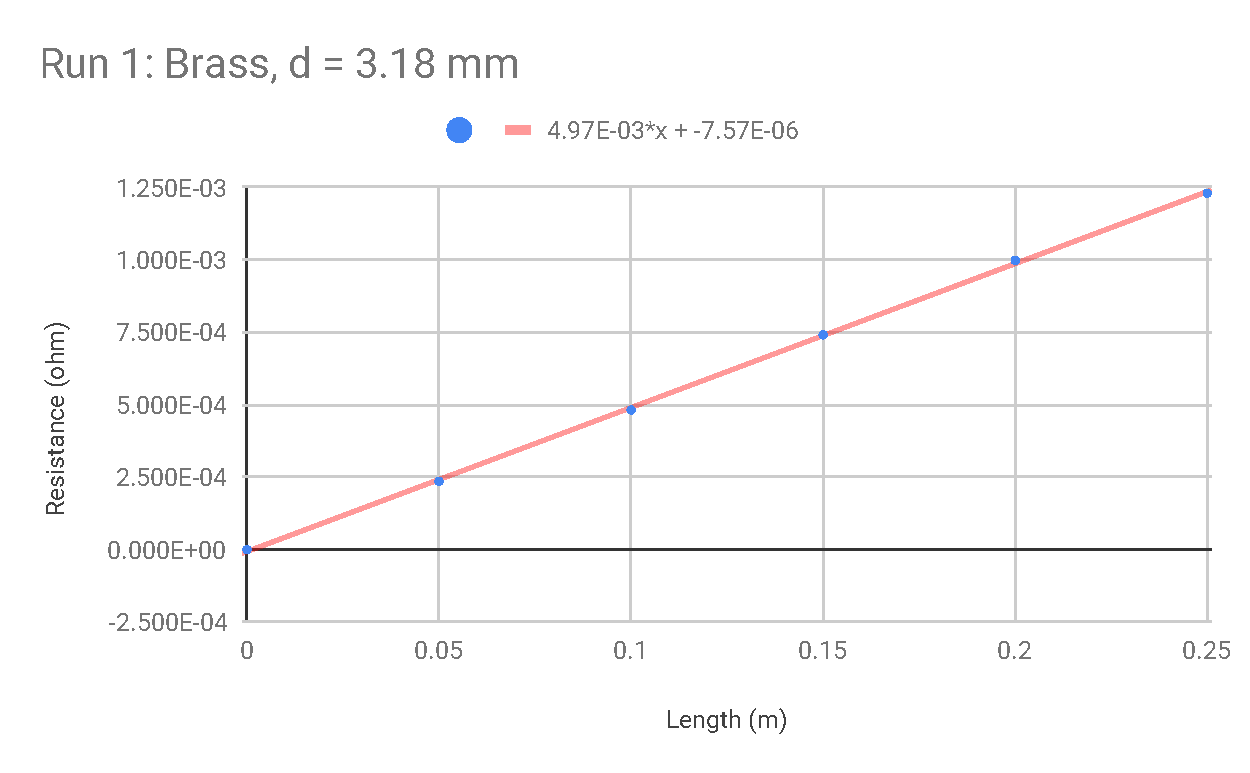
\includegraphics[scale=0.74]{image/02-resistance/run1.pdf}
	\caption{Run 1}
	\label{figure.02.run.1}
\end{figure}
%
\begin{figure}[ht]
	\centering
	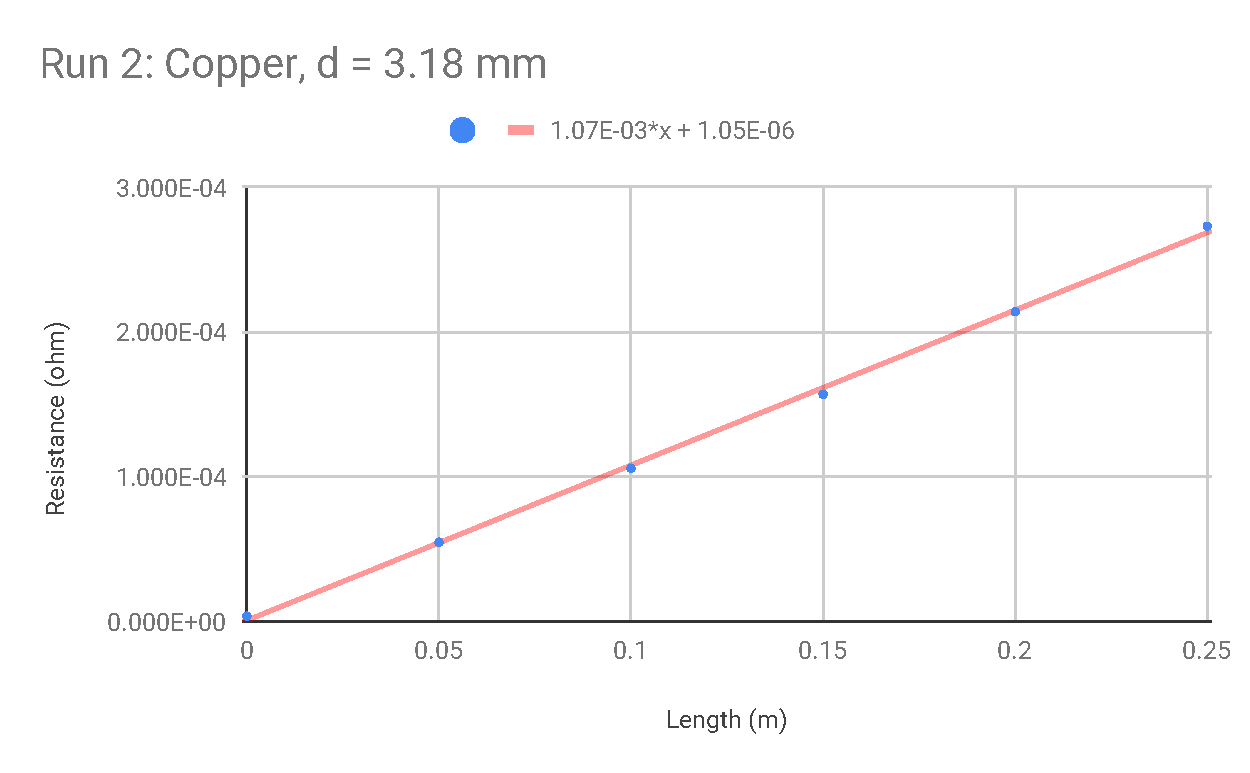
\includegraphics[scale=0.74]{image/02-resistance/run2.pdf}
	\caption{Run 2}
	\label{figure.02.run.2}
\end{figure}
%
\begin{figure}[ht]
	\centering
	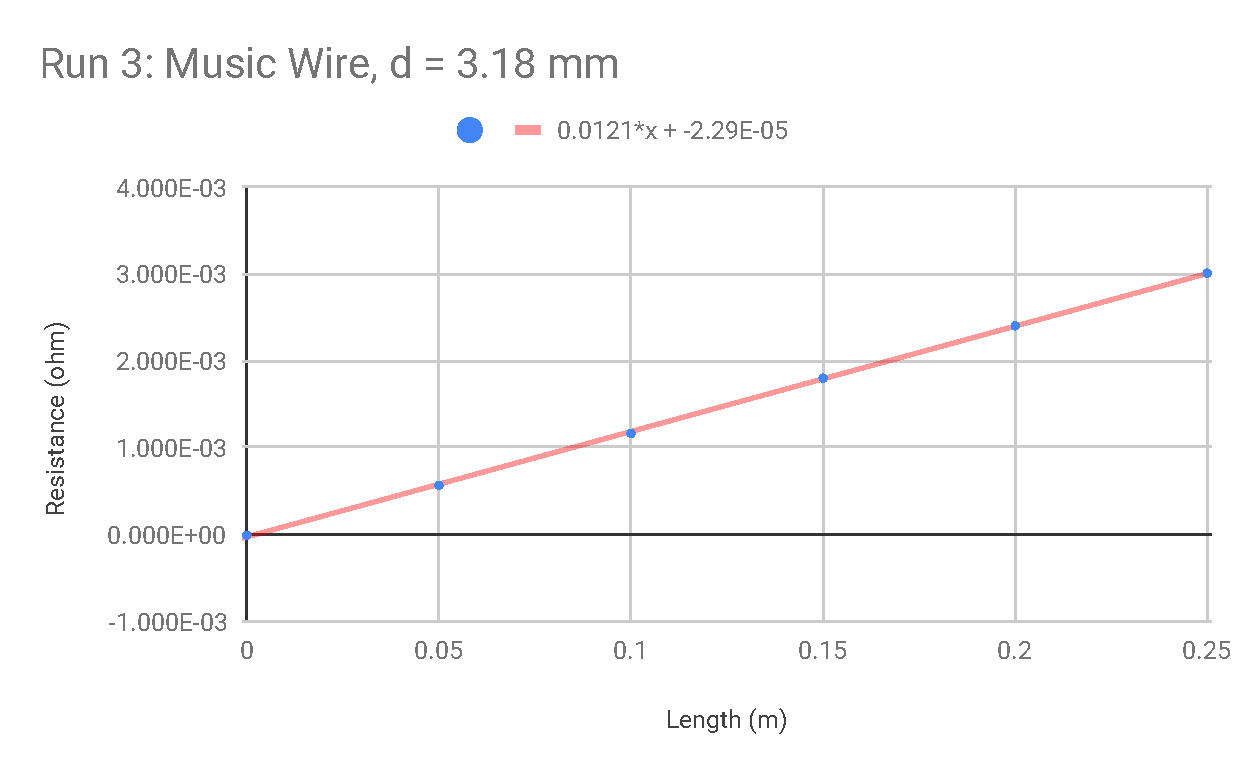
\includegraphics[scale=0.74]{image/02-resistance/run3.pdf}
	\caption{Run 3}
	\label{figure.02.run.3}
\end{figure}
%
\begin{figure}[ht]
	\centering
	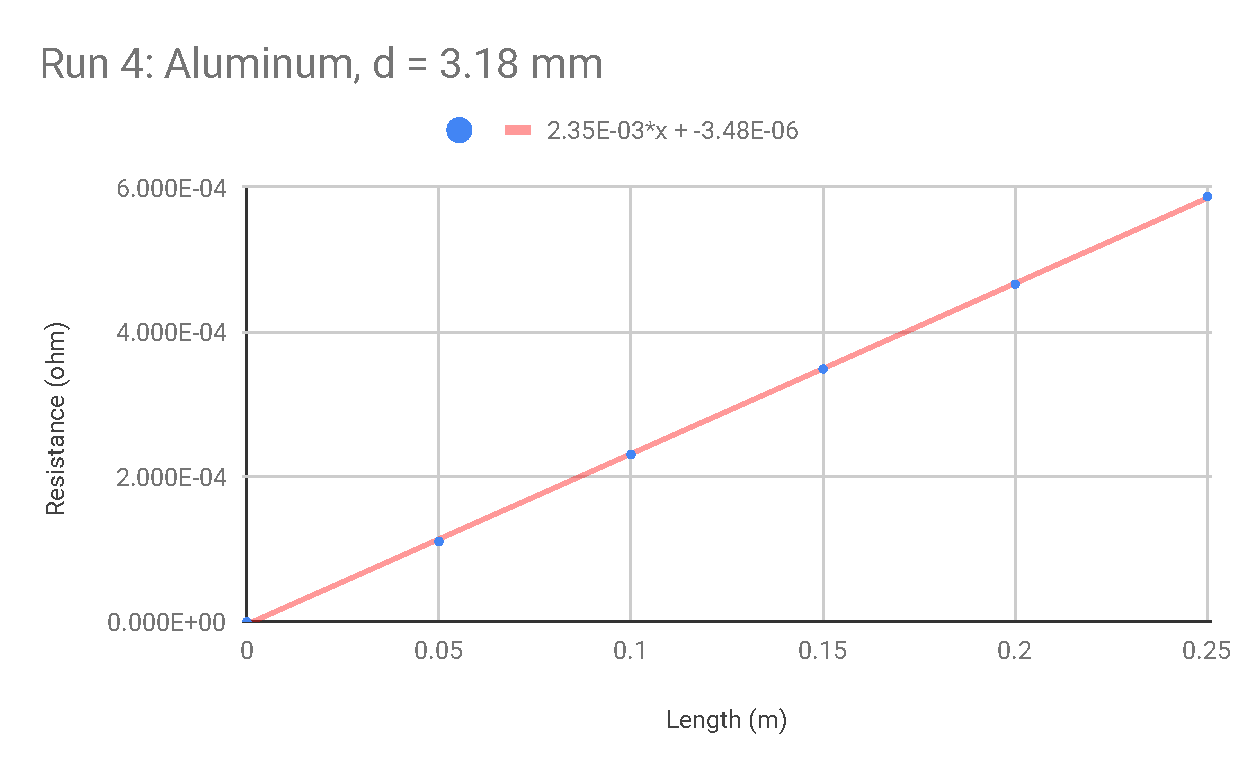
\includegraphics[scale=0.74]{image/02-resistance/run4.pdf}
	\caption{Run 4}
	\label{figure.02.run.4}
\end{figure}
%
\begin{figure}[ht]
	\centering
	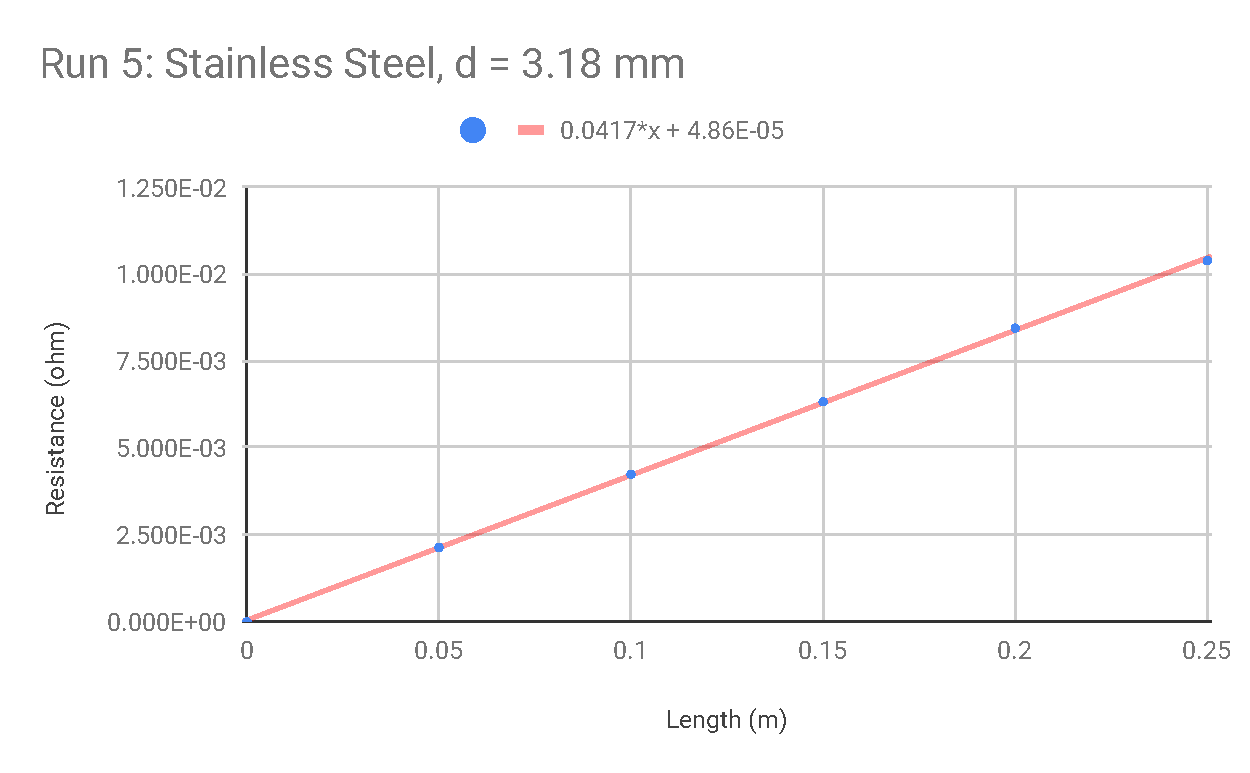
\includegraphics[scale=0.74]{image/02-resistance/run5.pdf}
	\caption{Run 5}
	\label{figure.02.run.5}
\end{figure}
%
\begin{figure}[ht]
	\centering
	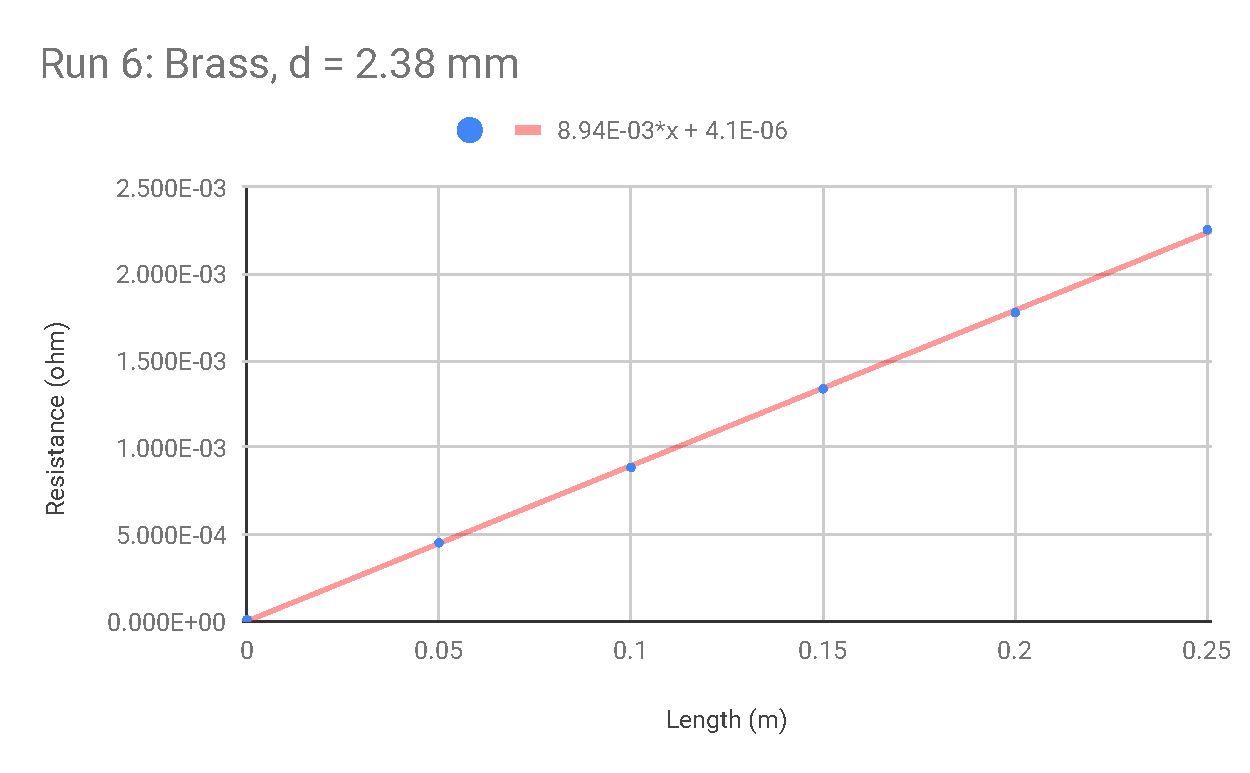
\includegraphics[scale=0.74]{image/02-resistance/run6.pdf}
	\caption{Run 6}
	\label{figure.02.run.6}
\end{figure}
%
\begin{figure}[ht]
	\centering
	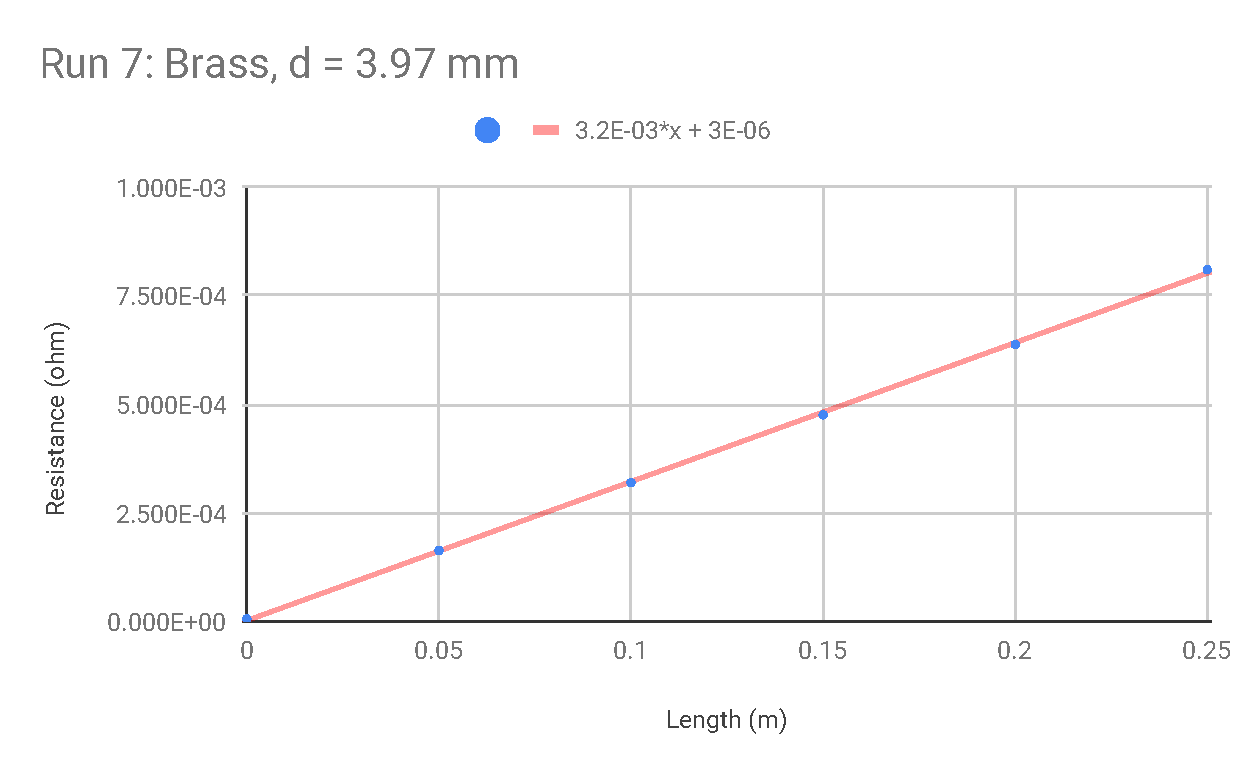
\includegraphics[scale=0.74]{image/02-resistance/run7.pdf}
	\caption{Run 7}
	\label{figure.02.run.7}
\end{figure}
%
\begin{figure}[ht]
	\centering
	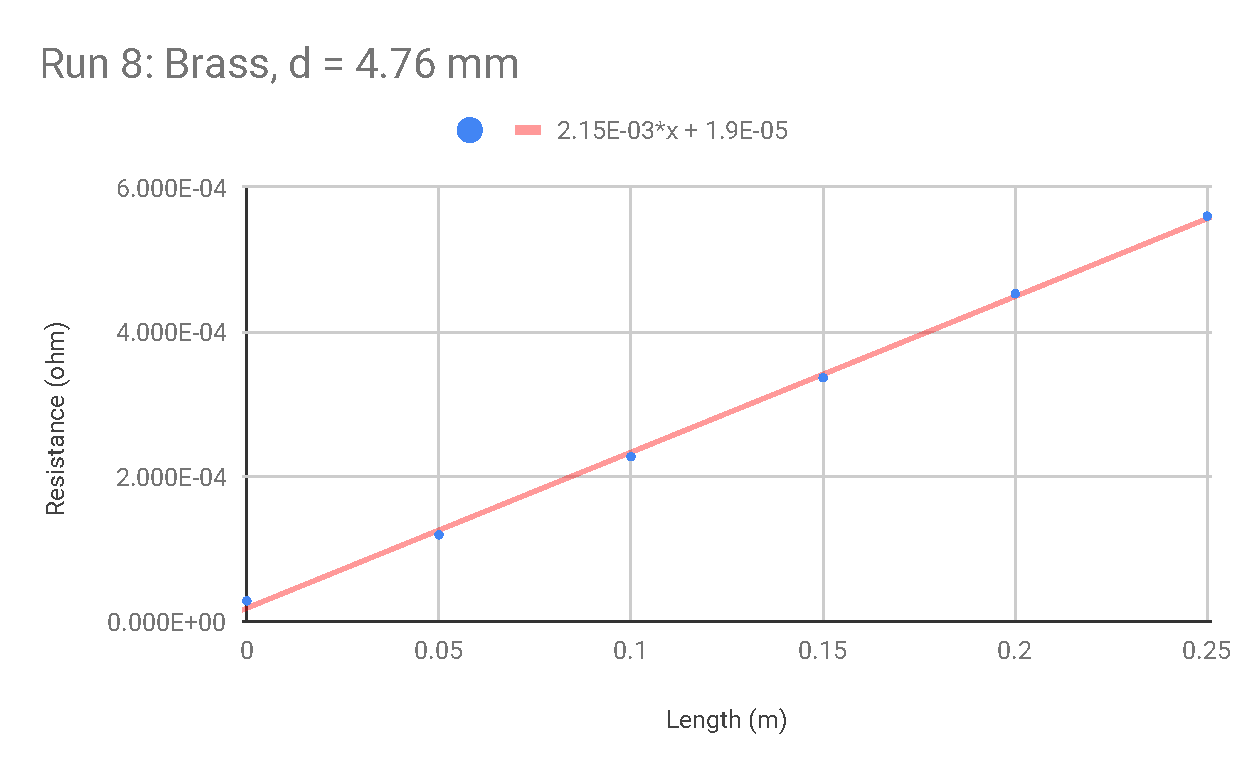
\includegraphics[scale=0.74]{image/02-resistance/run8.pdf}
	\caption{Run 8}
	\label{figure.02.run.8}
\end{figure}
%
\begin{figure}[ht]
	\centering
	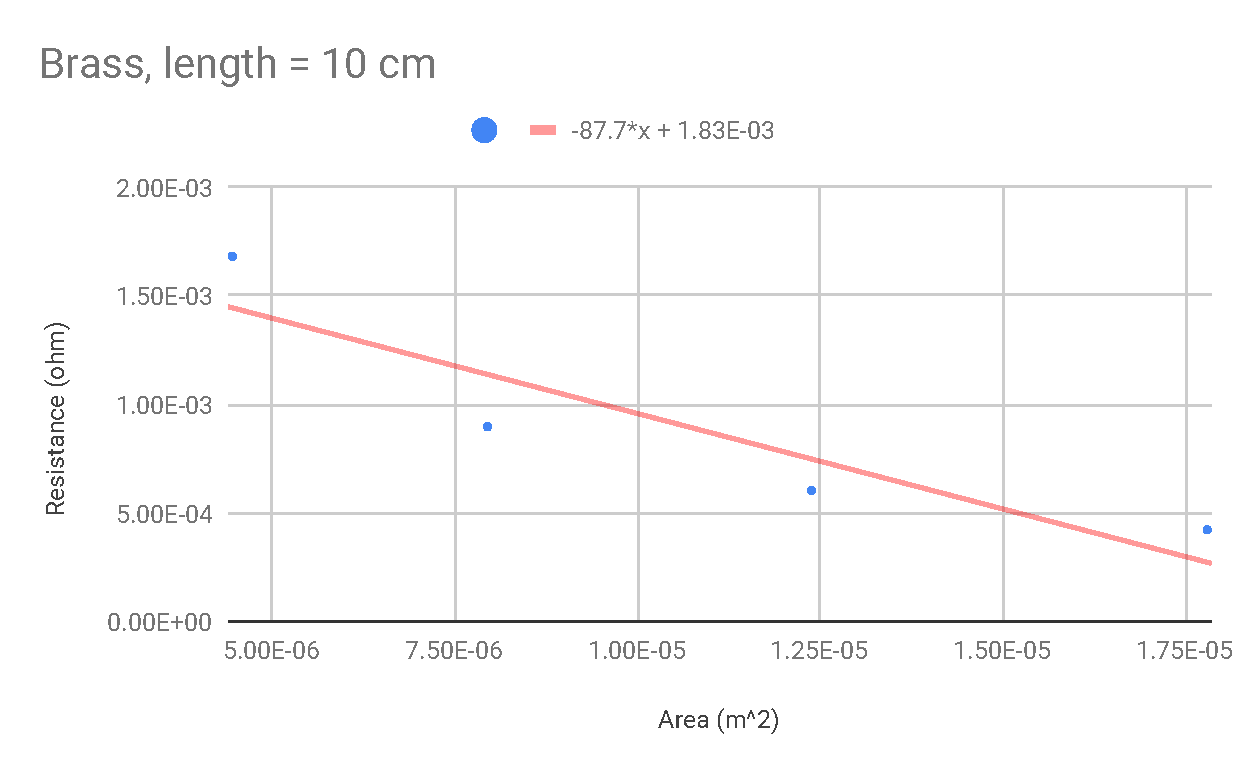
\includegraphics[scale=0.74]{image/02-resistance/10cm-non-linear.pdf}
	\caption{Brass, $l = 10$ cm, non-linear behavior}
	\label{figure.02.10cm.non.linear}
\end{figure}
%
\begin{figure}[ht]
	\centering
	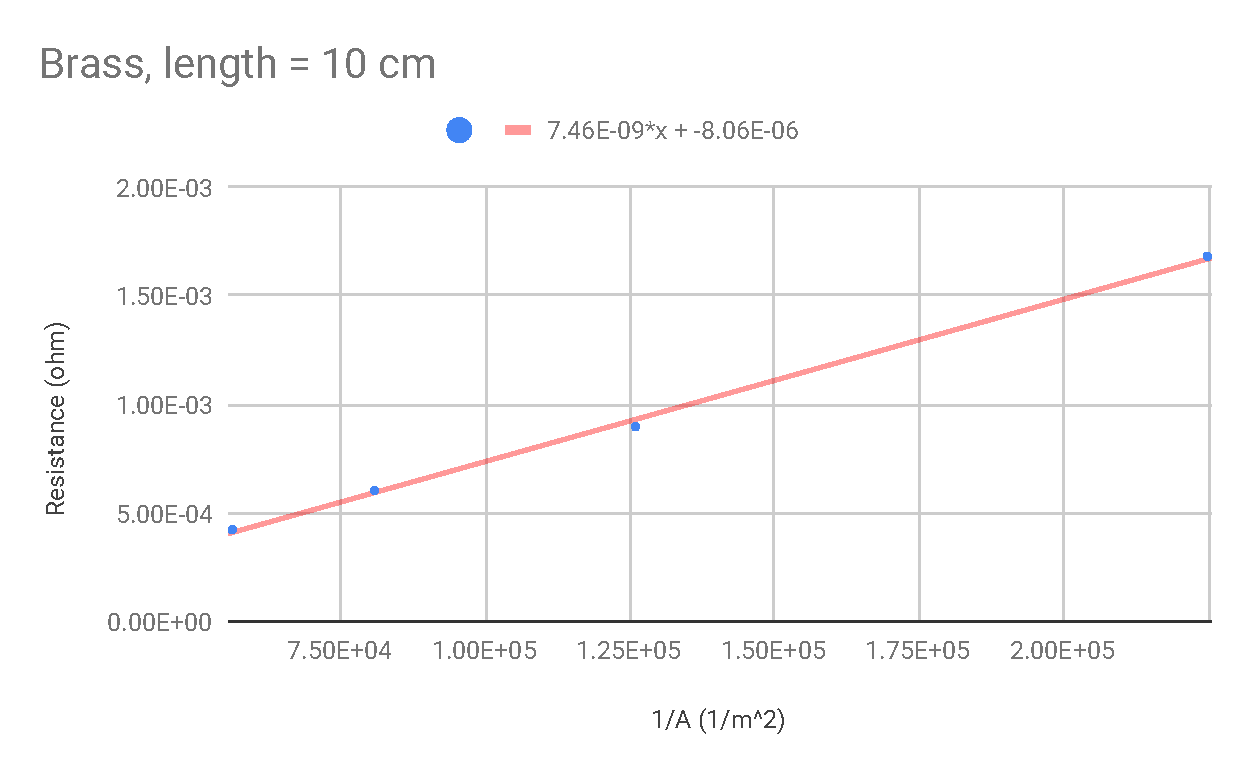
\includegraphics[scale=0.74]{image/02-resistance/10cm.pdf}
	\caption{Brass, $l = 10$ cm}
	\label{figure.02.10cm}
\end{figure}
%
\begin{figure}[ht]
	\centering
	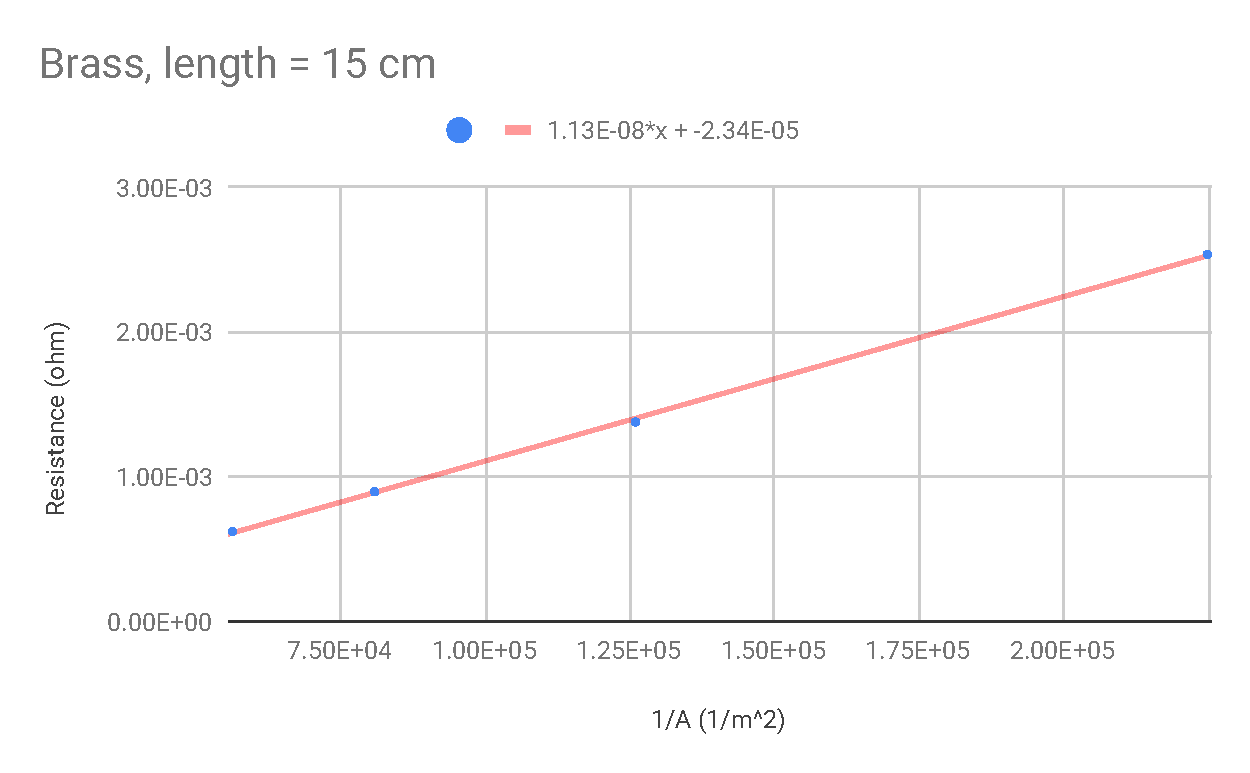
\includegraphics[scale=0.74]{image/02-resistance/15cm.pdf}
	\caption{Brass, $l = 15$ cm}
	\label{figure.02.15cm}
\end{figure}
%
\begin{figure}[ht]
	\centering
	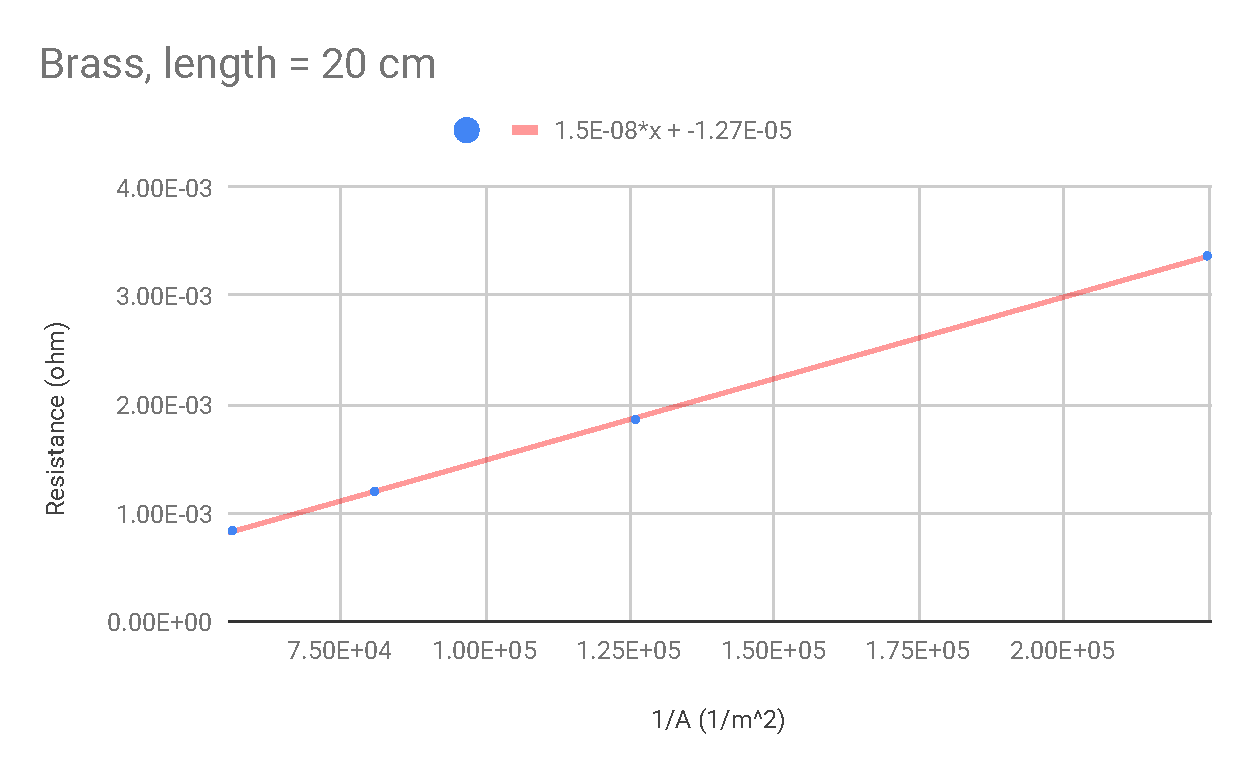
\includegraphics[scale=0.74]{image/02-resistance/20cm.pdf}
	\caption{Brass, $l = 20$ cm}
	\label{figure.02.20cm}
\end{figure}
%
\begin{figure}[ht]
	\centering
	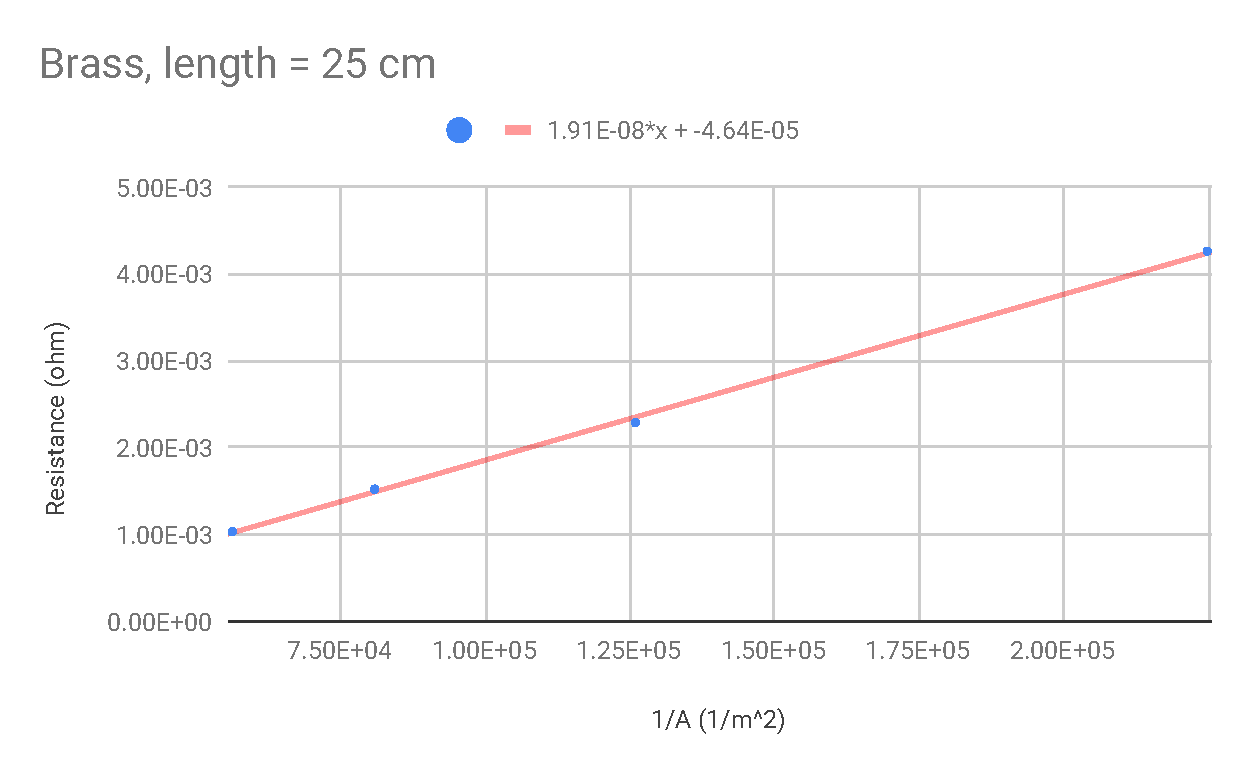
\includegraphics[scale=0.74]{image/02-resistance/25cm.pdf}
	\caption{Brass, $l = 25$ cm}
	\label{figure.02.25cm}
\end{figure}
%
